\documentclass[runningheads]{llncs}

\usepackage{graphicx}
\usepackage{amsmath}
\usepackage{booktabs}
\usepackage{array}
\usepackage{multirow}
\usepackage{enumitem}
\usepackage{url}
\usepackage{tabularx}
\usepackage[normalem]{ulem} % \sout for strike-through (must load before xcolor's \st)
\usepackage{xcolor}
\graphicspath{{figures/}{figures/latency/}{figures/latency/figures/}}
\urlstyle{rm}

\newcolumntype{P}[1]{>{\raggedright\arraybackslash}p{#1}}

% Compact numbered list for use inside a table cell: flush-left (labels align
% with the column header), no extra vertical margin, tight item spacing.
\newenvironment{cellsteps}
  {\begin{enumerate}[leftmargin=*,labelsep=0.4em,labelindent=0pt,
       topsep=0pt,partopsep=0pt,itemsep=1pt,parsep=0pt,label=\arabic*.]}
  {\end{enumerate}}

% ---------------------------------------------------------------------------
% Rebuttal revision markup. Flip \rebuttaltrue -> \rebuttalfalse for the
% camera-ready version: every macro below then renders as plain black text
% (and \rdel'd text disappears entirely).
% ---------------------------------------------------------------------------
\newif\ifrebuttal
\rebuttaltrue % <-- set to \rebuttalfalse for the final / camera-ready build

\definecolor{revadd}{HTML}{1A6DCC}  % blue  -- newly added / rewritten text
\definecolor{revdel}{HTML}{C0392B}  % red   -- text being removed

% Camera-ready fill-in marker: facts only the authors can supply (ethics board,
% approval number, participant demographics). Replace every \todofill{...} with
% the real value before submission; the red box makes leftovers impossible to miss.
\newcommand{\todofill}[1]{\textcolor{red}{\textbf{[#1]}}}

\ifrebuttal
  %... : new or rewritten passage (blue)
  \newcommand{\radd}[1]{\textcolor{revadd}{#1}}
  %  : text marked for deletion (red strike-through)
  \newcommand{\rdel}[1]{\textcolor{revdel}{\sout{#1}}}
  % new : replace old (red strike) with new (blue)
  \newcommand{\rrep}[2]{\rdel{#1}\,\radd{#2}}
\else
  \newcommand{\radd}[1]{#1}
  \newcommand{\rdel}[1]{}
  \newcommand{\rrep}[2]{#2}
\fi

\begin{document}

\title{UnifiedXRMotion: A Schema-Parameterized Validity-Aware Runtime Contract for Heterogeneous XR Avatar Motion}
\titlerunning{UnifiedXRMotion}
\author{Anonymous Authors}
\authorrunning{Anonymous Authors}
\institute{Paper under double-blind review}
\maketitle

\begin{abstract}
	XR avatar-motion pipelines increasingly combine directly observed tracking, vision-based landmarks, inferred body motion, replay streams, synthetic inputs, and retargeted outputs. These producers differ not only in body coverage, joint layout, and coordinate convention, but also in which pose components are available at each slot. UnifiedXRMotion explores a simple systems design decision: make component availability first-class runtime data, separate from component values. A producer publishes values into a schema-defined skeletal representation and marks which components are available; a consumer reads region views and gates access using those availability bits rather than source-specific records. Observed, inferred, replayed, synthetic, and retargeted components flow through the same representation, while provenance remains implicit in the producing node rather than encoded in the data record. Evaluation follows this contract boundary from implementation evidence to selected producers, reusable consumers, representative producer-to-consumer paths, and a within-subjects setup-burden study. The results support a scoped systems contribution: explicit component availability can connect heterogeneous XR avatar-motion producers to reusable downstream consumers without requiring those consumers to depend on SDK-specific motion records.
	\keywords{Extended reality \and Avatar motion \and Tracking middleware \and Motion-data contract \and Runtime systems \and Authoring}
\end{abstract}

\section{Introduction}\label{sec:introduction}
XR avatars depend on motion pipelines that span tracking acquisition, skeletal representation, motion processing, retargeting, recording, optional transport, and rendering. In practice these stages are often tied to one SDK or one avatar asset. A hand tracker may expose a vendor-specific joint order; a body tracker may report only a subset of joints; a vision model may provide positions but not reliable rotations; a replay stream may preserve previously recorded availability; and an inference or retargeting node may publish components that were not directly observed. This heterogeneity is not merely inconvenient engineering. It makes it hard to replace trackers, compare pipelines, record and replay motion, or reuse downstream avatar consumers without rewriting glue code.

Existing XR APIs and tracking middleware address important parts of this problem. OpenXR standardizes access to XR devices and extensions such as hand tracking~\cite{khronos_openxr_1_0,openxr_ext_hand}. Earlier VR middleware, including VRPN~\cite{taylor2001vrpn}, OpenTracker~\cite{reitmayr2001openarchitecture}, and Ubiquitous Tracking~\cite{newman2004ubiquitous}, showed that device abstraction and distributed tracking are valuable architectural tools. UnifiedXRMotion builds on that lesson at a narrower layer: avatar-motion pipelines that must carry incomplete skeletal components through adapters, filters, inferred-motion producers, retargeters, record/replay utilities, and optional network wrappers.

The central design choice is to make \emph{component availability} explicit data, separate from both schema-defined slot identity and component values. UnifiedXRMotion does not prescribe a fixed skeleton or slot count. Instead, a pipeline instantiates the contract with a schema that defines addressable motion slots, parent relations, and region views; a producer publishes values for the slots and components it has available; each pose component is guarded by a validity bit; and downstream consumers read only the components whose bits are set. This contract does not assert that a component is ground-truth correct, directly measured, or high-confidence. It only states that the producing node has made that component available for downstream consumption under its own semantics. The evaluated prototype uses one body-and-hands schema instance, but the slot count is not part of the contract semantics.

This paper makes three contributions:
\begin{itemize}
	\item \textbf{Availability as first-class runtime data}: a schema-parameterized skeletal motion contract that separates slot identity and component values from per-component availability.
	\item \textbf{A heterogeneous producer and adapter boundary} that maps selected XR, vision, replay, synthetic, inferred-motion, and retargeted producers into the shared representation while localizing source-specific joint ordering, coordinate conversion, body coverage, and missing-component semantics.
	\item \textbf{A reusable authoring pattern with a scoped setup-burden benefit}: because heterogeneous producers share one availability-gated contract, hand and full-body tracking are configured through the same producer--retargeter--avatar pattern. A within-subjects study ($N=19$) provides initial evidence that, for the prepared Unity authoring task, this pattern lowers procedural setup burden relative to a vendor-SDK workflow (completion time, NASA-TLX, SUS).
\end{itemize}

\section{Related Work}\label{sec:related}
\paragraph{Tracking middleware and XR APIs.}
VRPN provides a device-independent and network-transparent interface for VR peripherals~\cite{taylor2001vrpn}. OpenTracker introduced a modular software architecture for tracking configurations~\cite{reitmayr2001openarchitecture}, and Ubiquitous Tracking modeled distributed spatial relationships as a graph of tracking transformations~\cite{newman2004ubiquitous}. OpenXR standardizes XR device access and extensions such as hand tracking~\cite{khronos_openxr_1_0,openxr_ext_hand}; platform SDKs add body, hand, controller, camera, or device-specific streams~\cite{meta_and_openxr_2025}. These systems abstract devices, transforms, or API access. UnifiedXRMotion instead targets a skeletal avatar-motion record in which individual pose components may be unavailable and consumers explicitly gate reads using component availability.

\paragraph{Avatar motion and XR authoring abstractions.}

  Avatar representation is central to embodiment and social presence in shared XR~\cite{yun2023animationfidelity,baker2021avatar,weidner2023avatarsagents}, and a growing body of work brings believable avatar motion into XR from different angles.
  Recent methods generate full-body motion from sparse tracking signals~\cite{jiang2022avatarposer,dai2024hmd,yang2021lobstr,starke2024categorical}, making avatar representation possible even from limited VR device tracking, while other works improve the usability of creating it: AvatarGo enables plug-and-play self-avatar setup~\cite{ponton2022avatargo}, and AR Patterns catalogs event-driven design patterns for XR authoring~\cite{ackermann2023arpatterns}.
  We share this motivation of bringing avatar representation into XR.
  Our particular interest is in letting various sources drive avatar representation through a single reusable pattern, and UnifiedXRMotion provides the reusable XR structure for this: component availability becomes runtime data in the motion contract rather than source-specific logic inside each consumer.





  In current practice, capabilities such as motion generation and avatar setup are typically implemented per pipeline, against a specific source, SDK, or rig.
  UnifiedXRMotion instead factors the source-specific part out into a shared runtime representation that producers publish into and consumers read from, so that supporting an additional source does not require rewriting downstream code.
By making per-component availability first-class in a shared runtime record, a consumer reads motion through the same view interface across source types, provided the producer and consumer agree on the schema and coordinate space.
In the spirit of middleware and interchange abstractions, the contribution is not a new estimator, retargeter, or interchange format, but a runtime contract that makes this boundary explicit and reusable.



Figure~\ref{fig:availability-boundary} illustrates the boundary with a heterogeneous pipeline. In a source-specific implementation, hand tracking, vision landmarks, lower-body inference, and replay streams expose different notions of coverage, missing components, tracking state, or inferred output; that logic leaks into downstream consumers. UnifiedXRMotion moves this logic to the contract boundary. Producers publish component values with availability bits, and retargeting, recording, transport, or visualization consumers read schema-defined views using availability-gated access.

\begin{figure}[t]
	\centering
	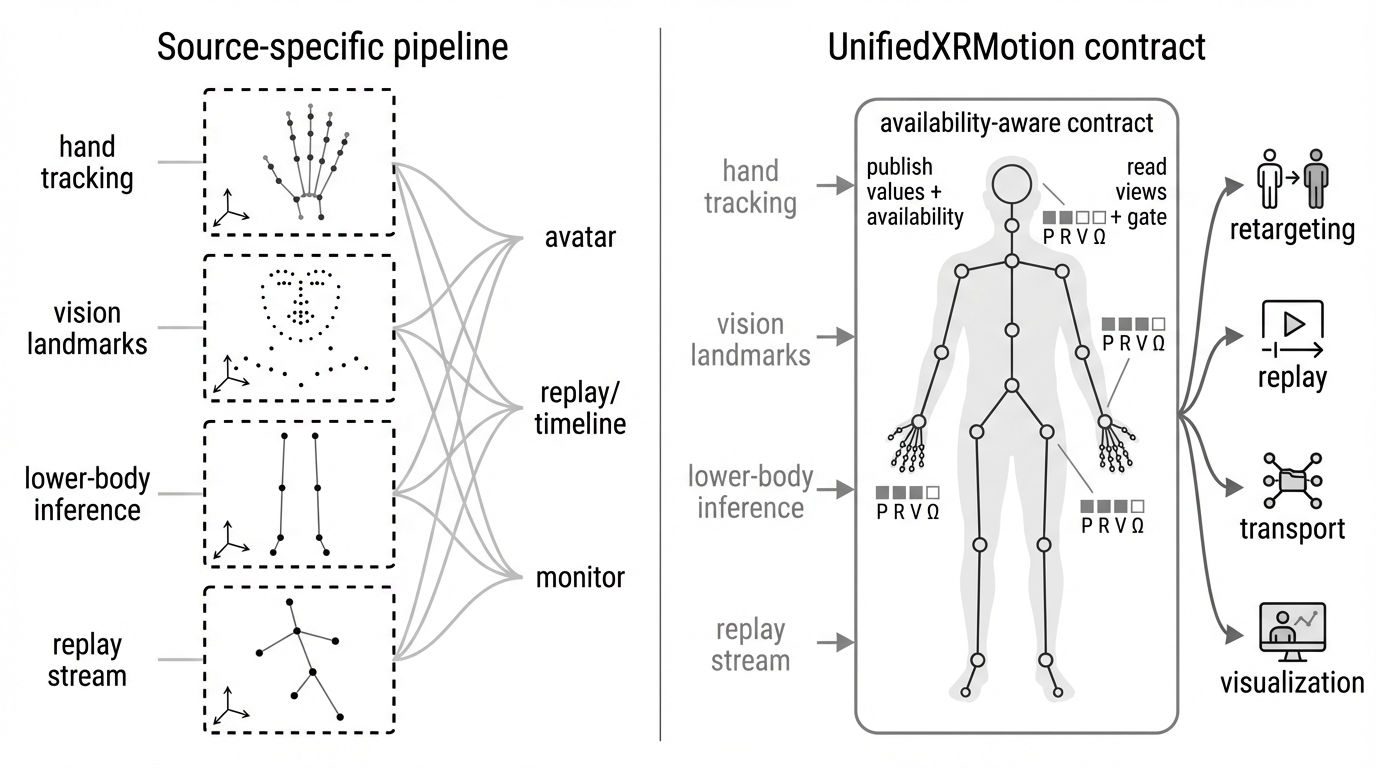
\includegraphics[width=0.86\textwidth]{figures/availability_boundary.png}
	\caption{Conceptual contrast for first-class component availability. Source-specific pipelines push missing-component logic into consumers, with small axis glyphs indicating source-specific coordinate and layout conventions. UnifiedXRMotion moves availability to the contract boundary: producers publish values and availability bits, and consumers read views using availability-gated access.}
	\label{fig:availability-boundary}
\end{figure}

\section{Validity-Aware Motion Contract}\label{sec:contract}
The central design decision in UnifiedXRMotion is to represent component availability as first-class runtime data, separate from component values. The contract instantiation that follows from this decision consists of a schema-parameterized address space, region views, per-slot pose records, and per-component availability flags. The contract does not require a fixed skeleton or slot count. Instead, a pipeline instantiates an active schema that defines slot identities, parent relations, and region views. A slot is a stable address in that schema, such as a head, wrist, fingertip, tracker, prop, facial control, or application-specific joint. Runtime samples then carry component values and availability bits for the slots in the active schema. This separation requires producer--consumer agreement on the active schema instance, and the current contract represents availability as a binary flag rather than continuous confidence.

A contract instance separates static schema from runtime state. Other applications may instantiate the same contract with different schemas, provided that producers and consumers agree on slot identities, region views, and component-availability semantics. The static schema is
\begin{equation}
	\mathcal{S}=(S,P,R,K),
\end{equation}
where $S=\{s_0,\ldots,s_{n-1}\}$ is a finite set of motion slots, $P$ is an optional parent relation, $R$ is a set of named region views with each $r_j\subseteq S$, and $K$ is the set of pose-component kinds. A runtime sample stores
\begin{equation}
	M=\{(m_i,V_i)\}_{i=0}^{n-1}, \qquad
	m_i=(p_i,q_i,v_i,\omega_i), \qquad
	V_i=(b^p_i,b^q_i,b^v_i,b^\omega_i),
\end{equation}
with $b_i^k\in\{0,1\}$. A consumer may read component $m_i^k$ only when $b_i^k=1$. The prototype implements this rule through \texttt{PhysicBone}, which stores pose fields and a \texttt{PoseFlag} bitmask, and through \texttt{KinematicBuffer<T>} and \texttt{BodyType} views over full-body, upper-body, lower-body, two-arm, two-hand, and hand regions.

%
Figure~\ref{fig:example} gives a concrete end-to-end instance.
Each participating node acts as an adapter boundary that exposes availability. 
Under a producer-consumer agreement, nodes exchange a shared kinematic buffer whose view exposes pose values gated by per-component availability within the same contract.
These nodes extend to a configurable pipeline.


\begin{figure}[t]
	\centering
	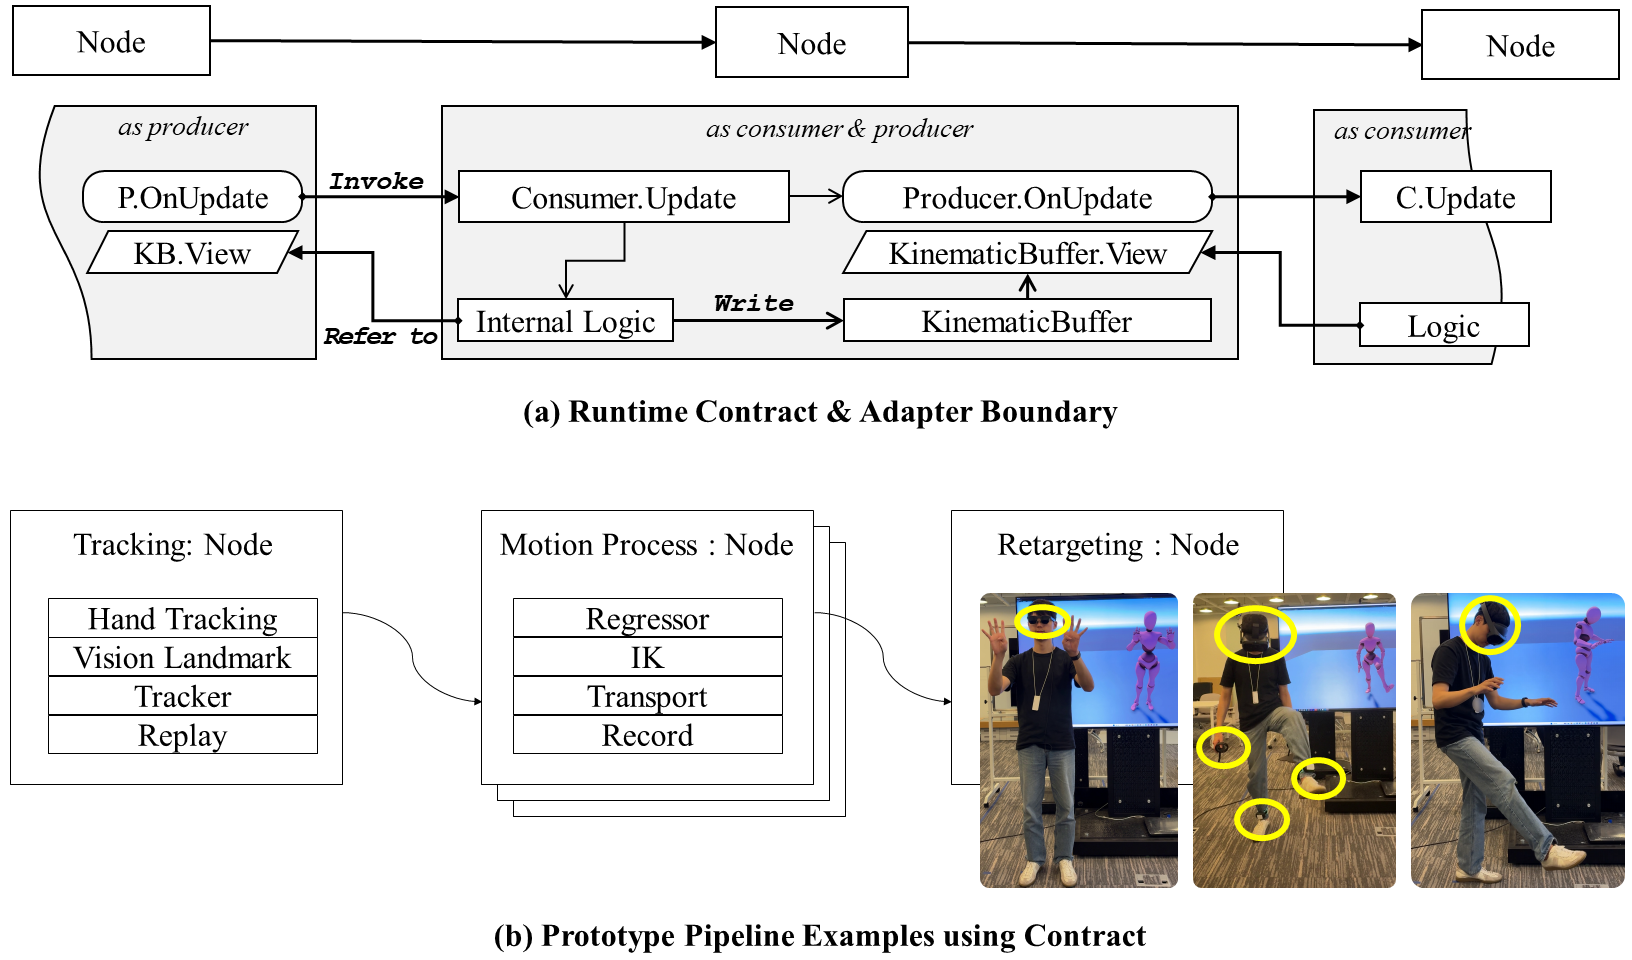
\includegraphics[width=\textwidth]{figures/figX-example.png}
  \caption{End-to-end pipeline under the contract. (a) Each node acts as an adapter boundary: a \emph{producer} publishes pose values and availability bits into its \texttt{KinematicBuffer<T>}, exposed through its buffer view;
a \emph{consumer} reads an upstream view through availability-gated access and may republish the result downstream after applying its internal logic.
(b) The same structure instantiated by concrete nodes (tracking, motion-processing, retargeting), with the retargeting node driving a custom avatar from tracked motion. Heterogeneous producers connect to the same downstream consumer through this contract rather than through source-specific records.}
	\label{fig:example}
\end{figure}

Table~\ref{tab:contract} maps the abstract contract definition to the prototype evidence used later in the paper. The table also states how each concept should be interpreted when it is used as evidence for the systems claim.

\begin{table}[t]
	\caption{Contract concepts and prototype evidence for the evaluated runtime contract.}\label{tab:contract}
	\centering
	\scriptsize
	\begin{tabular}{@{}P{23mm}P{48mm}P{48mm}@{}}
		\toprule
		Concept          & Prototype evidence                                                                                                   & Contract interpretation                                                                                                                  \\
		\midrule
		Schema and slots & Active schema instance with slot identities, parent maps, and region views.                                          & Slot count is not part of the contract semantics; pipelines require schema agreement and mappings.                                       \\
		Pose record      & Per-slot \texttt{PhysicBone} fields for position, rotation, velocity, scalar angular velocity, and local transforms. & The record carries component values and flags, but not timestamp, continuous confidence, or source provenance.                           \\
		Availability     & \texttt{PoseFlag} marks position, rotation, velocity, and angular-velocity availability per slot.                    & Availability denotes that a component is publishable under producer semantics, not that it is ground-truth correct or directly observed. \\
		Region views     & \texttt{KinematicBuffer<T>} and \texttt{BodyType} expose full-body, upper/lower-body, arms, hands, and hand views.   & Views preserve schema slot identity across body subsets; they are not discovered from arbitrary avatars.                                 \\
		Serialization    & Optional transport writes the flag first and can omit unavailable components.                                        & Transport preserves the contract semantics of partial records; compression is not the contribution evaluated here.                       \\
		\bottomrule
	\end{tabular}
\end{table}

The prototype enforces this contract through four operational obligations. Producers set availability flags for the components they publish into a slot. Consumers gate reads and assignments on those flags. Region views preserve slot identity across full-body, upper-body, lower-body, arm, and hand subsets (Figure~\ref{fig:contract}). Recording and optional transport preserve flags together with the published components. These obligations define how the following sections use evidence: adapter evidence is relevant at the publication boundary, and consumer evidence is relevant when downstream nodes actually gate reads through the published flags.

\begin{figure}[t]
	\centering
	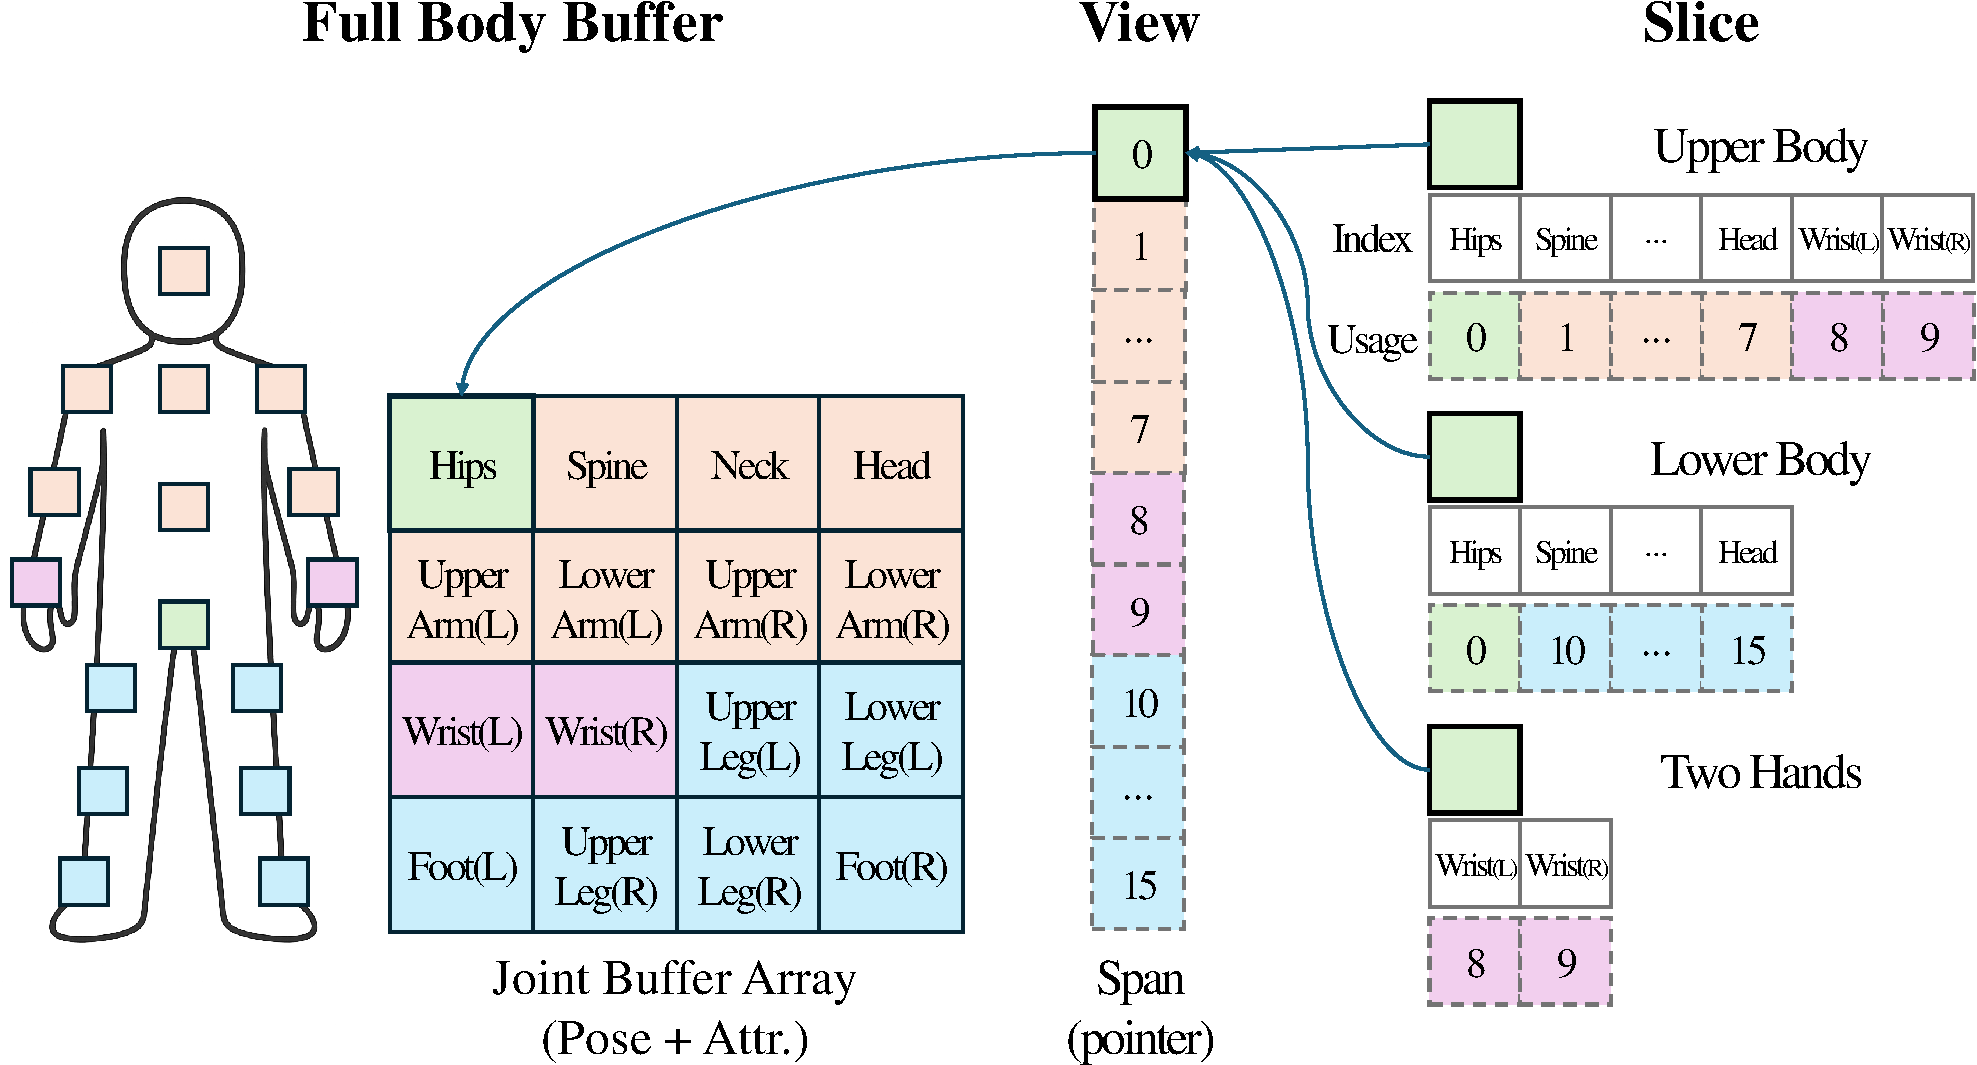
\includegraphics[width=0.94\textwidth]{fig2-kinematicbuffer.pdf}
	\caption{Prototype buffer and region-view instantiation of the contract. An active schema buffer is exposed through region views so that producers and consumers can operate on the subset they require without fixing the contract to one slot count.}
	\label{fig:contract}
\end{figure}

The same interpretation applies to inferred and retargeted motion. A lower-body inference node may publish a rotation as available, and a retargeting node may publish an avatar-specific component as available, but the contract does not encode whether that component was observed, inferred, reconstructed, replayed, or retargeted. Provenance is implicit in the producing node. Likewise, a vision adapter may threshold continuous confidence into a binary availability bit, but the continuous confidence value is not preserved in the current record.

\section{Heterogeneous Producers and Adapter Boundary}\label{sec:adapters}
Producers publish motion into the contract. Device and SDK adapters are the boundary where native tracking outputs become contract records. Each adapter initializes or reads a source, maps native joint ordering into schema slots, converts coordinate conventions where needed, marks component availability, and publishes pose records. The adapter code remains vendor-specific wrapper and conversion logic; the reusable artifact is the boundary after publication, where downstream nodes depend on slot identity and component availability rather than native SDK records.

The prototype exposes \texttt{ITrackingDeviceHandler}, a minimal adapter interface for initialization, tracked schema slots, a tracking-information buffer, and a tracking update. Its producer portfolio spans observed XR devices, MediaPipe vision sources, Android-AR or scene-transform sources, replay and synthetic streams, and representative inferred or retargeted producers. Table~\ref{tab:producers} summarizes where concrete source examples enter the shared representation and what remains adapter-side responsibility.

\begin{table}[t]
	\caption{Selected producer and adapter paths used to evaluate publication into the shared contract.}\label{tab:producers}
	\centering
	\scriptsize
	\begin{tabular}{@{}P{24mm}P{25mm}P{35mm}P{35mm}@{}}
		\toprule
		Producer family              & Source examples                                                                                     & Mapping into contract                                                                                            & Evaluation scope                                                                                      \\
		\midrule
		Observed XR devices          & Meta/OVR body and hand, Unity XR/OpenXR HMD, controller, and hand sources, Vive hands, XREAL hands. & Native joint IDs and device poses are mapped into full-body or region slots with per-component availability.     & Adapter logic is SDK-specific, and coverage is limited to selected source families.                   \\
		Vision sources               & MediaPipe upper-body and hand landmarks.                                                            & Landmark positions are mapped into hand or upper-body slots; visibility is thresholded into binary availability. & Continuous confidence is quantized away, and coordinate offsets remain adapter assumptions.           \\
		Replay and synthetic sources & Recorded \texttt{PhysicBone} arrays, transform sources, dummy or mouse-driven inputs.               & Publish the same slot records and flags as live sources.                                                         & Fidelity depends on the recorded stream or synthetic setup.                                           \\
		Inferred producers           & Codebook-style lower/upper-body regressors and filters.                                             & Publish inferred components back into contract buffers with availability flags.                                  & Inference algorithm and model quality are not contributions; provenance is not encoded in the record. \\
		Retargeted producers         & IK and retargeting nodes that fill avatar-motion regions.                                           & Consume views and may republish retargeted components into the same representation.                              & IK and retargeting methods are representative nodes rather than algorithmic novelty.                  \\
		\bottomrule
	\end{tabular}
\end{table}

The table supports the adapter-boundary claim: source-specific joint ordering, handedness and axis conversion, body-region coverage, missing velocity or angular-velocity channels, and SDK tracking-state or visibility conversion are handled before publication. Source-specific offsets, calibration assumptions, and confidence-to-bit thresholds remain part of adapter authoring; the shared record begins once values and availability have been published.

\section{Validity-Aware Consumers}\label{sec:consumers}
The strongest consumer evidence is the retargeting path. \texttt{RetargetSystem} reads \texttt{KinematicBufferView<PhysicBone>} instances and checks \texttt{PoseFlag} before assigning position or rotation to avatar transforms. If a component is unavailable, the assignment is skipped rather than silently using a default or stale source value. The same consumer dispatches across \texttt{BodyType} views such as full body, upper/lower body, two arms, and two hands, so the consuming code is organized around contract views rather than around a producing SDK.

The other downstream paths exercise the same access discipline. Recording and replay store and republish \texttt{PhysicBone} arrays with their flags, allowing replay to appear as another producer in the same representation. Optional network serialization writes the \texttt{PoseFlag} before optional channels so that partial records preserve availability semantics. Filters and inference nodes read upstream views, gate access through flags, and republish processed or inferred components. Across these consumers, the common pattern is not a shared algorithm but a shared contract: each node reads a schema-defined view and uses availability flags to decide which components may be consumed.

Table~\ref{tab:producer-consumer} is the central downstream-reuse evidence. It links the producer paths to the contract view consumed downstream, showing that different production paths can publish into the same record/view abstraction before consumers branch on availability and region view rather than on native SDK record format.

\begin{table}[t]
	\caption{Representative producer-to-consumer paths used to evaluate reuse through shared contract views.}\label{tab:producer-consumer}
	\centering
	\scriptsize
	\begin{tabular}{@{}P{28mm}P{24mm}P{28mm}P{39mm}@{}}
		\toprule
		Producer path               & Contract view                                    & Downstream consumer                   & Claim supported                                                                                                           \\
		\midrule
		Meta/OVR body tracking      & Full-body or upper/lower-body view               & Retargeting system                    & Vendor body streams can be consumed through schema views after adapter mapping.                                           \\
		UnityXR/OpenXR hand sources & Two-hands or hand view                           & Hand retargeting and recording        & Hand-only streams use the same slot/view structure as other producers.                                                    \\
		MediaPipe vision landmarks  & Position-available upper-body or hand view       & Filters, recorder, optional transport & Position-dominant vision sources can publish partial component availability without requiring special downstream records. \\
		Codebook-style inference    & Lower-body or full-body view                     & Retargeting and recorder              & Inferred components are consumed through the same view and flag discipline as observed components.                        \\
		Replay or synthetic source  & Recorded or generated \texttt{PhysicBone} buffer & Same consumers         & Replay and test inputs can act as producers without changing the consumer interface.                                      \\
		Retargeting or IK node      & Region view republished as a buffer              & Later recording or optional transport & Retargeted components can be republished and later recorded or transported through the same contract.                     \\
		\bottomrule
	\end{tabular}
\end{table}

Together, these paths support the medium-paper reuse claim: heterogeneous producers terminate their source-specific logic at adapters, and reusable consumers operate on shared contract views with availability-gated reads. The evidence is illustrative rather than exhaustive; some concrete adapters and retargeters remain vendor-specific by design.

\section{Prototype Implementation}\label{sec:implementation}
UnifiedXRMotion is implemented as a Unity package. Motion slots are stored in preallocated buffers; region views expose subsets without requiring a separate representation for each body part. Root producers are advanced by a frame-driven trigger list, and motion updates propagate through sender/receiver events. This runtime organization is a Unity-oriented composition mechanism rather than a general graph scheduler or graph optimizer.

This implementation realizes the contract concepts in Table~\ref{tab:contract}: buffers store slot records and flags, region views expose schema-defined subsets, and update paths preserve availability across producer and consumer boundaries.

At runtime, a producer updates a contract buffer for the active schema instance. Device adapters fill directly observed components, replay nodes copy recorded records, inference nodes publish estimated components, and retargeting nodes may republish transformed components into another region view. Updates are propagated through explicit sender/receiver events rather than through a global scheduler. Within each producer-triggered update path, downstream receivers consume the buffer state published by the upstream node during that event propagation. Global graph scheduling, cross-frame synchronization, out-of-order reconciliation, provenance tracking, and automatic schema negotiation are outside the scoped contract claim.

The package includes representative nodes for filtering, IK, retargeting, inference, recording, replay, and optional FishNet-based transport~\cite{fishnet}. The included IK nodes use FABRIK~\cite{aristidou2011fabrik}, and the inference nodes build on codebook-style control~\cite{starke2024categorical}. The contribution here is that these nodes can consume or publish the same validity-aware representation. Optional transport preserves flags and available components, but transport is treated as implementation support rather than the center of the paper.

\section{Evaluation and Case Study Evidence}\label{sec:evaluation}

The evaluation has two purposes.
	First, whether component availability is instantiated in a working runtime contract.
	Second, whether the authoring workflow built on this contract reduces the procedural setup burden in the prepared Unity task.

It does not evaluate tracking accuracy, retargeting quality, broad device coverage, display-response timing, or general developer productivity.

\paragraph{Traceability of implementation evidence.}
	The implementation evidence is organized as a traceability chain rather than as isolated summaries.
	Table~\ref{tab:contract}  identifies the contract elements and their interpretation.
	The operational obligations in Section~\ref{sec:contract} define how producers, consumers, views, recording, and transport must use availability flags.
	Table~\ref{tab:producers} shows where heterogeneous source families enter the contract.
	Table~\ref{tab:producer-consumer} then links representative producer paths to possibly reusable downstream contract views.

\paragraph{Setup-burden study.}

	We conducted a within-subjects Unity study to assess whether the contract-based workflow reduces avatar setup burden.
	Nineteen participants took part (aged \todofill{age range / mean age}; \todofill{$n$ women, $n$ men}), recruited from \todofill{recruitment population, e.g., researchers and graduate students at the authors' institution}.
	This pool was chosen to be representative of the framework's intended users---developers who configure XR avatar pipelines in a game engine---rather than of end users: on 5-point Likert scales, mean self-reported experience was 3.21 ($SD=0.92$) for programming and 2.84 ($SD=1.01$) for XR and game engines, indicating intermediate proficiency.
	The study protocol was approved by \todofill{name of ethics review board} (approval no.~\todofill{number}).
	All participants provided informed consent and were compensated.
	The study compares a UnifiedXRMotion workflow against a vendor-SDK workflow, each mapping user tracking to a custom avatar.
	Within each workflow, participants performed two subtasks sequentially: (1) Custom-Hands and (2) Full-Body mapping.
	Three controls keep the comparison fair.
	Condition order (UnifiedXRMotion-first vs.\ vendor-SDK-first) was counterbalanced across participants to mitigate order effects.
	All trials ran in a controlled desktop XR simulator, so setup effort is not confounded with on-device build and deployment latency.
	For Custom-Hands, hand-axis tuning was pre-completed in the vendor-SDK workflow; UnifiedXRMotion handles this within the adapter boundary, so participants performed it in neither condition.
	The study used Unity 6000.0.33f1 with Meta Core, Movement SDK, and XR Simulator 78.0.0.

\paragraph{Hypotheses and measures.}
	The study tested three directional hypotheses: relative to the vendor-SDK workflow, the UnifiedXRMotion workflow yields (H1) lower task completion time, (H2) lower perceived workload, and (H3) higher perceived usability.
	The corresponding measures were: \emph{completion time}, in seconds from task start to the verified end state (participants compared their scene behavior against reference clips and the administrator confirmed completion); \emph{workload}, as the raw NASA--TLX score, i.e., the mean of the six subscales on 0--100 scales with the performance subscale reversed so that higher values consistently indicate higher workload; and \emph{usability}, as the System Usability Scale (SUS) score on 0--100.
	Presentation order (UnifiedXRMotion first, AB, $n=10$; vendor SDK first, BA, $n=9$) was retained as a between-subjects factor in the analysis to test for order effects.

Participants were instructed to prioritize correctness and completion rather than speed. We therefore interpret completion time as procedural setup burden for the tested task, not as a general developer-speed estimate. The procedure also excludes adapter authoring and full integration of a previously unseen hand mesh.

\begin{table}[t]
	\caption{Task procedure comparison of the workflows (study task guide,
			verbatim; cross-checked against the official vendor-SDK manuals). 
      UnifiedXRMotion repeats one \emph{avatar\,$\to$\,producer\,$\to$\,retargeter\,$\to$\,connect} pattern for both regions; the vendor SDK uses different mechanisms for hands and body, several repeated per hand, and the body wizards expand to multi-stage
			editors (italicized stages). Hand-axis retargeting was pre-completed for the
			vendor SDK, so it doesn't appear in the column.}
	\label{tab:task-procedure}
	\centering
	\scriptsize
	\setlength{\tabcolsep}{4pt}
	\renewcommand{\arraystretch}{1.1}
	\begin{tabularx}{\textwidth}{@{}>{\raggedright\arraybackslash}X >{\raggedright\arraybackslash}X@{}}
		\toprule
		UnifiedXRMotion (Task A) & Vendor SDK (Task B) \\
		\midrule
		\multicolumn{2}{@{}l}{\textbf{Hands}} \\
		\addlinespace[2pt]
		\begin{cellsteps}
		     \item Attach \texttt{Motion\,Avatar} to a custom hand avatar
		     \item Set \texttt{Body\,Type\,=\,Two\,Hands}
		     \item Add \texttt{MotionSystem} prefab
		     \item Add producer; add retargeter
		     \item Add retargeter to \texttt{Input\,Motions}; set \texttt{Input\,Motion}
		   \end{cellsteps}
		 & \begin{cellsteps}
		     \item Add \texttt{OVRCameraRig} to scene root
		     \item Add \texttt{OVRInteractionComprehensive}; keep \texttt{OVRHands}; set rig ref
		     \item Add synthetic hands (\texttt{OVRLeftHandSynthetic}, \texttt{OVRRightHandSynthetic})
		     \item Delete the default hand visuals
		     \item Reparent custom hand meshes (L, R)
		     \item Configure hand visuals, per hand
		     \item Bind \texttt{Source\,=\,OVRHands}, per hand
		   \end{cellsteps} \\
		\midrule
		\multicolumn{2}{@{}l}{\textbf{Body}} \\
		\addlinespace[2pt]
		\begin{cellsteps}
		     \item Attach \texttt{Motion\,Avatar} to a custom humanoid avatar
		     \item Add \texttt{MotionSystem} prefab
		     \item Add producer; add retargeter
		     \item Add retargeter to \texttt{Input\,Motions}; set \texttt{Input\,Motion}
		   \end{cellsteps}
		 & \begin{cellsteps}
		     \item Set \texttt{OVRManager} body-tracking flags
		     \item Run the Retargeting Config.\ Editor wizard \textit{(T-Pose, Min/Max align, scale, validate)}
		     \item Add a Character Retargeter \textit{(+ \texttt{OVRBody}, skeleton type; per-joint twist optional)}
		   \end{cellsteps} \\
		\midrule
		\multicolumn{2}{@{}l}{\textbf{Pattern}} \\
		\addlinespace[2pt]
		One reused pattern (hands = body) & Two mechanisms (hands $\neq$ body); 3 authoring surfaces \\
		\bottomrule
	\end{tabularx}
\end{table}


	To clarify the guided tasks used in the study, Table~\ref{tab:task-procedure}
	decomposes the participant protocol into setup steps for each condition.
	UnifiedXRMotion satisfies both hands and full body through one reused
	producer--retargeter--avatar pattern, whereas the vendor SDK requires different
	mechanisms per body region.


\begin{table}[t]
	\caption{Descriptive statistics of the setup-burden study ($N=19$): mean $\pm$ standard deviation per condition, overall and by presentation order (AB: UnifiedXRMotion first, $n=10$; BA: vendor SDK first, $n=9$). NASA--TLX is the raw 0--100 workload score after reversing the performance subscale so that higher values consistently indicate higher workload. Inferential statistics are reported in the text.}
	\label{tab:user-results}
	\centering
	\scriptsize
	\setlength{\tabcolsep}{3.5pt}
	\renewcommand{\arraystretch}{1.08}
	\begin{tabularx}{\textwidth}{@{}>{\raggedright\arraybackslash}X
		>{\centering\arraybackslash}p{28mm}
		>{\centering\arraybackslash}p{24mm}
		>{\centering\arraybackslash}p{23mm}@{}}
		\toprule
		Condition ($M\!\pm\!SD$) & Completion time (s)   & NASA--TLX & SUS \\
		\midrule
		UnifiedXRMotion, all
		          & $564.03\!\pm\!176.58$
		          & $30.53\!\pm\!17.55$
		          & $73.42\!\pm\!17.08$                     \\
		Vendor SDK, all
		          & $972.89\!\pm\!243.36$
		          & $49.74\!\pm\!18.29$
		          & $34.47\!\pm\!13.91$                     \\
		\addlinespace[2pt]
		UnifiedXRMotion, order AB
		          & $550.20\!\pm\!216.52$
		          & $34.58\!\pm\!21.49$
		          & $72.75\!\pm\!21.71$                     \\
		Vendor SDK, order AB
		          & $857.80\!\pm\!199.51$
		          & $54.58\!\pm\!19.50$
		          & $27.00\!\pm\!9.04$                      \\
		\addlinespace[2pt]
		UnifiedXRMotion, order BA
		          & $579.40\!\pm\!130.06$
		          & $26.02\!\pm\!11.42$
		          & $74.17\!\pm\!11.18$                     \\
		Vendor SDK, order BA
		          & $1100.78\!\pm\!231.35$
		          & $44.35\!\pm\!16.22$
		          & $42.78\!\pm\!14.00$                     \\
		\bottomrule
	\end{tabularx}

	\vspace{2pt}
	{\footnotesize Statistics are computed from the supplied raw CSVs. The study supports setup burden in this prepared task; it does not establish general developer productivity or long-term maintainability.\par}
\end{table}

\paragraph{Analysis and results.}
Table~\ref{tab:user-results} reports the descriptive statistics.
Each measure was analyzed with a $2\times2$ mixed ANOVA with condition (UnifiedXRMotion vs.\ vendor SDK) as the within-subjects factor and presentation order (AB vs.\ BA) as the between-subjects factor; with two levels per factor, sphericity is not at issue.
Test assumptions were verified beforehand: Shapiro--Wilk tests did not reject normality of the paired condition differences for any measure, either overall (all $W\ge.974$, $p\ge.859$) or within each order group (all $p\ge.297$), and Levene tests indicated homogeneous variances of the differences across order groups (all $p\ge.330$).
Nonparametric Wilcoxon signed-rank tests agreed with every parametric conclusion reported below (all $p<.001$).

The main effect of condition was significant for all three measures, supporting H1--H3: completion time was lower under UnifiedXRMotion ($F(1,17)=161.07$, $p<.0001$, $\eta_p^2=.90$; $M_{\mathrm{diff}}=-408.9$~s, 95\% CI $[-493.3,\,-324.5]$, paired $t(18)=-10.18$, Hedges' $g_{\mathrm{av}}=-1.84$), NASA--TLX workload was lower ($F(1,17)=48.27$, $p<.0001$, $\eta_p^2=.74$; $M_{\mathrm{diff}}=-19.2$, 95\% CI $[-24.9,\,-13.6]$, $t(18)=-7.13$, $g_{\mathrm{av}}=-1.03$), and SUS was higher ($F(1,17)=68.27$, $p<.0001$, $\eta_p^2=.80$; $M_{\mathrm{diff}}=+38.9$, 95\% CI $[28.7,\,49.2]$, $t(18)=7.98$, $g_{\mathrm{av}}=+2.39$).
The main effect of order was not significant for any measure (completion time: $F(1,17)=2.54$, $p=.130$; NASA--TLX: $F(1,17)=1.50$, $p=.238$; SUS: $F(1,17)=3.01$, $p=.101$).
The condition$\times$order interaction was significant for completion time ($F(1,17)=10.98$, $p=.0041$, $\eta_p^2=.39$) but not for NASA--TLX ($F(1,17)=0.09$, $p=.767$) or SUS ($F(1,17)=2.31$, $p=.147$).

\paragraph{Order effect on completion time.}
To quantify the relative impacts behind this interaction, we fitted a linear mixed-effects regression of completion time on condition, order, and their interaction, with a random intercept per participant (reference: vendor SDK, order AB).
The estimated UnifiedXRMotion advantage was $-307.6$~s ($SE=42.0$, $p<.0001$) in the AB order and $213.8$~s larger ($SE=61.0$, $p=.0005$) in the BA order.
Simple effects show that the interaction reflects an asymmetric practice effect: the vendor-SDK condition was faster when performed second, after participants had already completed the same task with UnifiedXRMotion ($857.80$ vs.\ $1100.78$~s; Welch $t(15.94)=2.44$, $p=.027$), whereas UnifiedXRMotion completion times were insensitive to position ($550.20$ vs.\ $579.40$~s; $t(14.96)=-0.36$, $p=.724$).
The UnifiedXRMotion advantage remained significant within both order groups (AB: $-307.6$~s, $t(9)=-6.76$, $p<.001$; BA: $-521.4$~s, $t(8)=-11.46$, $p<.001$), so the direction of the completion-time effect is order-robust while its magnitude is order-dependent.

Because the magnitude of the timing difference depends on presentation order, it should not be interpreted as a stable estimate of general developer productivity. The results support the narrower claim that, in this controlled Unity setup task, the contract-based workflow reduced the procedural configuration burden required from participants, with converging evidence from completion time, workload, and usability ratings.

\section{Discussion and Limitations}\label{sec:discussion-limitations}
UnifiedXRMotion is an implemented in-memory runtime contract, not a standardized interchange format or an end-to-end performance system. The evaluation therefore does not measure tracker latency, display-response timing, end-to-end frame budget, or offloading performance. The core record does not encode provenance, continuous confidence, schema version, or full timestamp propagation. Provenance is implicit in the producing node, so a downstream consumer cannot tell from the data record alone whether a component was directly observed, inferred, replayed, reconstructed, or retargeted. Vision confidence is collapsed into binary availability in the current adapters, losing information that future versions should preserve.

The adapter portfolio is selected rather than exhaustive. Each new tracker still requires a schema mapping, coordinate conversion, and validation, and some mappings contain source-specific assumptions such as offsets or calibration conventions. The evaluated body-and-hands schema is one prototype instance, not a general avatar skeleton or a required slot layout. Other pipelines may instantiate different schemas, but producers and consumers must agree on slot identities, region views, and mappings to avatar-specific rigs. The included IK, retargeting, filtering, and codebook-style modules are representative nodes, not algorithmic contributions.

The setup study also has limited scope. Hand-axis alignment and mesh-specific retargeting were pre-completed, participants worked on a prepared Unity task, and the study did not measure adapter-authoring effort, long-term maintenance, or quality of produced motion. Optional local/remote traces and transport utilities characterize application-level runtime behavior only; they should not be interpreted as display-response timing, remote-execution performance benefit, or user-perceived responsiveness.

\paragraph{Artifact availability.}
We will provide an anonymized Unity package, example scenes, analysis scripts, and the study materials used in the paper for review or upon acceptance, subject to the submission policy.

\section{Conclusion}\label{sec:conclusion}
UnifiedXRMotion presents component availability as first-class runtime data for heterogeneous XR avatar-motion pipelines. Producers publish observed, inferred, replayed, synthetic, or retargeted components into a shared schema-defined representation, and consumers read explicitly available components through region views. The Unity prototype demonstrates the contract with selected producer families, adapter mappings, reusable retargeting/recording/transport consumers, and a controlled setup-burden study. The contribution is a scoped but coherent contract design: explicit component availability can connect heterogeneous motion producers to reusable avatar-motion consumers.

\bibliographystyle{splncs04}
\bibliography{bib/references}
\end{document}
